% !TEX encoding = UTF-8
% !TEX TS-program = pdflatex
% !TEX root = ../tesi.tex

%**************************************************************
\chapter{Analisi dei requisiti}
\label{cap:analisi dei requisiti}
%**************************************************************

\intro{In questo capitolo vengono trattati le analisi dei requisiti del modulo di front-end della web-app, con i vari casi d'uso ed elenco dei requisiti. Infine vengono elencati i requisiti richiesti dall'azienda.}\\

%**************************************************************
\section{Descrizione generale}
\subsection{interfacce della web-app}
\subsubsection{Interfaccia menù}
L'utente può visualizzare il menù di un ristorante dopo aver scansionato il QR-code di un ristorante presente sul tavolo. Il menù è composto da un insieme di categorie, in cui ci sono tutti i piatti appartenenti a quella categoria. I piatti sono ordinati in base al suo id che è un numero univoco dentro ogni menù.
\subsubsection{Interfaccia lista ordini}
L'utente può vedere i piatti ordinati del suo tavolo di appartenenza, dove ci sono anche i piatti ordinati dalle altre persone del tavolo, inoltre può vedere i suoi piatti personali e i piatti in arrivo.
\subsubsection{Interfaccia gestione tavolo}
In questa maschera utente può creare una sessione di tavolo se non appartiene ad nessuna sessione, altrimenti può visualizzare il QR-code della sua sessione in modo da fare entrare gli altri nella sua sessione di tavolo.
\subsubsection{Interfaccia area personale}
Qui l'utente può effetture la login, di seguito se ha degli allergeni potrà inserire degli ingredienti nella blacklist in modo tale di non visualizzare i piatti contenenti quegli ingredienti nella sezione menù.
\subsection{Caratteristiche degli Utenti}
In questa sezione vengono descritti tutte le Caratteristiche degli utenti che possono utilizzare la web-app.
\subsubsection{Utente non autenticato}
Con il termine utente non autenticato ci si riferisce ad una qualsiasi persona non autenticata nel sistema, che può sfruttare le funzionalità di base offerte dalla piattaforma, ossia:
\begin{itemize}
    \item Visualizzare il menù del ristorante;
    \item Visualizzare i singoli piatti in modalità dettaglio;
    \item Creare una sessione di tavolo;
    \item Unire ad una sessione di tavolo già esistente;
    \item Uscire dalla sessione di tavolo;
    \item Aggiungere piatti negli ordini;
    \item Aggiungere note ai piatti ordinati;
    \item Spostare ordini in arrivo;
    \item Marcare i piatti in arrivo come arrivato;
    \item Registrare nella piattaforma;
    \item Effettuare la login.
\end{itemize}
\subsubsection{Utente autenticato}
Invece, con il termine “utente autenticato” ci si riferisce ad una persona registrata nel database e che ha effettuato l'accesso nella piattaforma, la quale, oltre a sfruttare le funzionalità dell'utente non autenticato, può anche:
\begin{itemize}
    \item Aggiungere piatti nei preferiti;
    \item Rimuovere piatti dai preferiti;
    \item Dare una recensione ad un piatto;
    \item Aggiungere ingredienti non voluti;
    \item Rimuovere gli ingredienti non voluti;
    \item Visualizzare la lista dei preferiti;
    \item Effettuare logout.
\end{itemize}
%**************************************************************
\subsection{Tecnologie utilizzate}
Per sviluppare la piattaforma verranno utilizzare le seguenti tecnologie:
\begin{itemize}
    \item Angular: per la creazione dell'interfaccia utente;
    \item HTML5: per creare la struttura dell'interfaccia untente;
    \item CSS3: per lo stile dell'interfaccia, viene utilizzato la sintassi SCSS;
    \item Stoplight: per simulare le chiamate Rest API;
    \item Angular Material: per la creazione dei componenti.
\end{itemize}
\subsection{Descrizione delle tecnologie}
\subsubsection{Angular}
Angular è un framework open source per sviluppare applicazioni web, permette di dividere l'applicazione in più componenti, grazie a questo è possibile riutilizzare lo stesso modulo in più parti della web-app, oltre a questo garantisce una maggiore manutenibilità e espandibilità.
\begin{figure}[H]
    \centering
    
\includegraphics[scale=0.1]{angular.png}
    \caption{Logo di Angular}
\end{figure}
\subsubsection{HTML5}
L'HyperText Markup Language, noto come HTML, è un linguaggio di markup più popolare, utilizzato per progettare le strutture dei siti web. Viene utilizzato da Angular per creare la struttura iniziale per le varie interfacce, poi queste strutture vengono modificate da Angular per generare la pagina dinamicamente. 
\begin{figure}[H]
    \centering
    
\includegraphics[scale=0.5]{html css.png}
    \caption{Logo di HTML e CSS}
\end{figure}
\subsubsection{CSS3}
Il CSS, sigla di Cascading Style Sheets, è il linguaggio utilizzato per modificare il layout delle pagine web, le regole vengono applicate nel ordine in cui vengono scritte. Per il progetto è stato utilizzato una sua estensione SCSS, la quale è compatibile con tutte le versioni di CSS. Tramite la SCSS è possibile dichiarare le regole CSS in blocchi quindi ci aiuta a scrivere regole CSS in più velocemente e comprensibile.
\subsubsection{TypeScript}
TypeScript è un linguaggio di programmazione open source sviluppato da Microsoft, che estende il classico JavaScript quindi qualsiasi codice scritto in JavaScript è anche eseguibile con TypeScript direttamente senza nessuna modifica. TypeScript rende molto più flessibile e flessibile JavaScript aggiungendo la firma dei metodi, classi, tipi di dato e tanto altro, grazie a queste caratteristiche utilizzando TypeScript ci ganrantisce controlli automatici, rilevando in automatico i bug prima della compilazione.
\subsubsection{Stoplight}
Stoplight è una piattaforma che offre la possibilità di progettare le API velocemente, grazie alla sua interfaccia user friendly. Offre un buon spazio per collabolare con gli altri, condividendo tutte le API con le sue descrizioni e risposte in modo chiaro.
\begin{figure}[H]
    \centering
    
\includegraphics[scale=0.4]{stoplight logo.png}
    \caption{Logo di Stoplight}
\end{figure}
\subsubsection{Angular Material}
Angular Material è un insieme di componenti UI già implementati, questi componenti possono essere direttamente utilizzati in Angular. Tutti i componenti offerti sono già responsive e sono facili da customizzare con le proprie preferenze, come il colore dei bottoni.
\begin{figure}[H]
    \centering
    
\includegraphics[scale=0.3]{angular material.png}
    \caption{Logo di Angular Material}
\end{figure}
\section{Casi D'uso}
\subsection{Introduzione }
In questa sezione verranno presentati i casi d'uso individuati durante la fase di analisi dei requisiti, i quali fanno riferimento a tutte le funzionalità che la web-app SushiLab dovrà offrire ad ogni utente che vorrà interfacciarsi con essa.
\subsection{Attori primari}
\begin{itemize}
    \item Utente non Autenticato: utente che non ha ancora effettuato la fase di autenticazione sulla piattaforma. Può essere in possesso o meno delle credenziali per l'autenticazione. Avrà funzionalità limitate rispetto ad un utente autenticato;
    \item Utente Autenticato: utente che ha effettuato l'autenticazione alla piattaforma tramite le proprie credenziali. Ha accesso ad ogni funzionalità messa a disposizione dalla piattaforma;
    \item  Utente Generico: può essere sia un utente autenticato che un utente non autenticato.
\end{itemize}
\subsection{Utente generico}
\subsection{UC1 - Visualizza menù}
\begin{figure}[H]
    \centering
    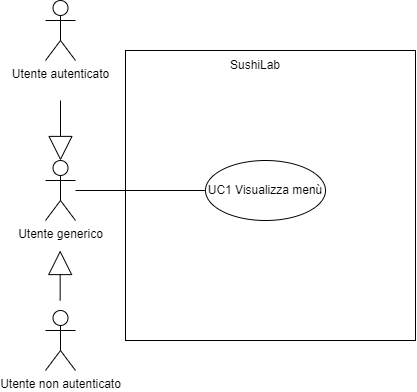
\includegraphics[scale=0.5]{usecase/tesi-uc1.drawio.png}
    \caption{Use Case - UC 1}
\end{figure}
\begin{itemize}
    \item \textbf{Descrizione:} L'utente visualizza il menù del ristorante.
    \item \textbf{Attore Primario:} Untente generico.
    \item \textbf{Precondizione:} L'utente si trova dentro la web-app sushiLab.
    \item \textbf{Postcondizione:} Viene visualizzato il menù del ristorante.
    \item \textbf{Scenrio principale:}
    \begin{itemize}
        \item L'utente si trova dentro il sistema;
        \item L'utente clicca sul bottone menù;
        \item Viene mostra il menù del ristorante.
    \end{itemize}
\end{itemize}
\subsection{UC1.1 - Visualizza categorie}
\begin{figure}[H]
    \centering
    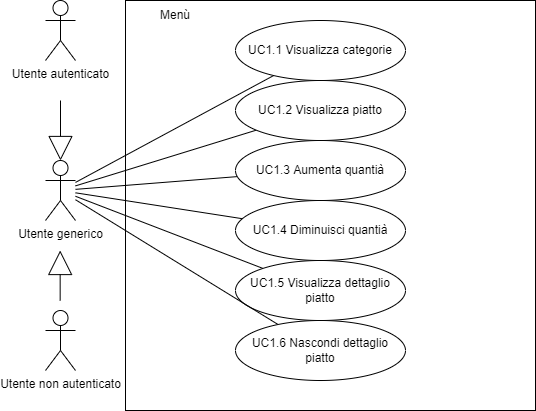
\includegraphics[scale=0.5]{usecase/tesi-uc11.drawio.png}
    \caption{Use Case - UC 1.1, UC 1.2, UC 1.3, UC 1.4, UC 1.5, UC 1.6}
\end{figure}
\begin{itemize}
    \item \textbf{Descrizione:} L'utente visualizza le categorie del menù.
    \item \textbf{Attore Primario:} Untente generico.
    \item \textbf{Precondizione:} L'utente si trova dentro la sezione menù.
    \item \textbf{Postcondizione:} Viene visualizzato i nomi delle categorie.
    \item \textbf{Scenrio principale:}
    \begin{itemize}
        \item L'utente si trova sezione menù;
        \item Viene mostrato le categorie del menù.
    \end{itemize}
\end{itemize}
\subsection{UC1.2 - Visualizza piatto}
\begin{itemize}
    \item \textbf{Descrizione:} L'utente visualizza i piatti del menù mostrando il numero, nome, prezzo, ingredienti, allergeni, limatazioni e la quantità. La quantità di default è 0 che indica che non è ancora stato ordinato.
    \item \textbf{Attore Primario:} Untente generico.
    \item \textbf{Precondizione:} L'utente si trova dentro la sezione menù.
    \item \textbf{Postcondizione:} Viene visualizzato i piatti del menù.
    \item \textbf{Scenrio principale:}  
    \begin{itemize}
        \item L'utente si trova sezione menù;
        \item Viene mostrato i piatti del menù.
    \end{itemize}
\end{itemize}
\subsection{UC1.3 - Aumenta quantità}
\begin{itemize}
    \item \textbf{Descrizione:} L'utente aumenta la quantità di un piatto.
    \item \textbf{Attore Primario:} Untente generico.
    \item \textbf{Precondizione:} L'utente si trova dentro la sezione menù o lista degli ordini personali.
    \item \textbf{Postcondizione:} Viene aggiunto il piatto specifico con la quantità aggiornata negli ordini.
    \item \textbf{Scenrio principale:}
    \begin{itemize}
        \item L'utente si trova sezione menù;
        \item L'utente clicca sul bottone + di un piatto;
        \item Viene aggiunto il piatto negli ordini.
    \end{itemize}
    \item \textbf{Scenrio alternativo:}
    \begin{itemize}
        \item L'utente si trova sezione menù o lista degli ordini personali;
        \item L'utente clicca sul bottone + di un piatto che è già presente negli ordini;
        \item Viene aumentato la quantità del piatto negli ordini.
    \end{itemize}
\end{itemize}
\subsection{UC1.4 - Diminuisci quantità}
\begin{itemize}
    \item \textbf{Descrizione:} L'utente dimiuisce la quantità di un piatto.
    \item \textbf{Attore Primario:} Untente generico.
    \item \textbf{Precondizione:} L'utente si trova dentro la sezione menù o lista degli ordini personali.
    \item \textbf{Postcondizione:} Viene dimiuito la quantità del piatto specifico negli ordini.
    \item \textbf{Scenrio principale:}
    \begin{itemize}
        \item L'utente si trova sezione menù o lista degli ordini personali;
        \item L'utente clicca sul bottone - di un piatto con quantità maggiore di 1;
        \item Viene diminuito la quantità del piatto negli ordini.
    \end{itemize}
    \item \textbf{Scenrio alternativo:}
    \begin{itemize}
        \item L'utente si trova sezione menù o lista degli ordini personali;
        \item L'utente clicca sul bottone - di un piatto con quantità uguale a 1;
        \item Viene rimosso il piatto dagli ordini.
    \end{itemize}
\end{itemize}
\subsection{UC1.5 - Visualizza dettaglio piatto}
\begin{itemize}
    \item \textbf{Descrizione:} L'utente visualizza i dettagli di un piatto nel menù, mostrando la recensione del piatto e il text-box per inserire una nota.
    \item \textbf{Attore Primario:} Untente generico.
    \item \textbf{Precondizione:} L'utente si trova dentro la sezione menù.
    \item \textbf{Postcondizione:} Viene visualizzato i dettagli di un piatto specifico.
    \item \textbf{Scenrio principale:}  
    \begin{itemize}
        \item L'utente si trova sezione menù;
        \item L'utente clicca sul bottom mostra dettagli;
        \item Viene mostrato i dettagli di un piatto.
    \end{itemize}
\end{itemize}
\subsection{UC1.6 - Nascondi dettaglio piatto}
\begin{itemize}
    \item \textbf{Descrizione:} L'utente nasconde i dettagli di un piatto specifico.
    \item \textbf{Attore Primario:} Untente generico.
    \item \textbf{Precondizione:} L'utente si trova dentro la sezione menù con un piatto in modalità dettaglio.
    \item \textbf{Postcondizione:} Viene nascosto i dettagli del piatto specifico.
    \item \textbf{Scenrio principale:}  
    \begin{itemize}
        \item L'utente si trova sezione menù;
        \item L'utente clicca sul bottom nascondi dettagli;
        \item Viene nascosto i dettagli del piatto.
    \end{itemize}
\end{itemize}
\subsection{UC2 - Gestione tavolo}
\begin{figure}[H]
    \centering
    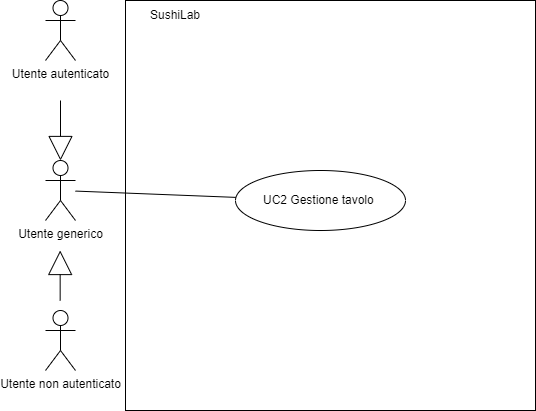
\includegraphics[scale=0.5]{usecase/tesi-uc2.drawio.png}
    \caption{Use Case - UC 2}
\end{figure}
\begin{itemize}
    \item \textbf{Descrizione:} L'utente visualizza la maschera di gestione tavolo.
    \item \textbf{Attore Primario:} Untente generico.
    \item \textbf{Precondizione:} L'utente si trova dentro la web-app sushiLab.
    \item \textbf{Postcondizione:} Viene visualizzato la maschera di gestione tavolo.
    \item \textbf{Scenrio principale:}
    \begin{itemize}
        \item L'utente si trova dentro il sistema;
        \item L'utente clicca sul bottone gestione tavolo nella navbar;
        \item Viene mostrato la maschera di gestione tavolo.
    \end{itemize}
\end{itemize}
\subsection{UC2.1 - Generazione sessione tavolo}
\begin{figure}[H]
    \centering
    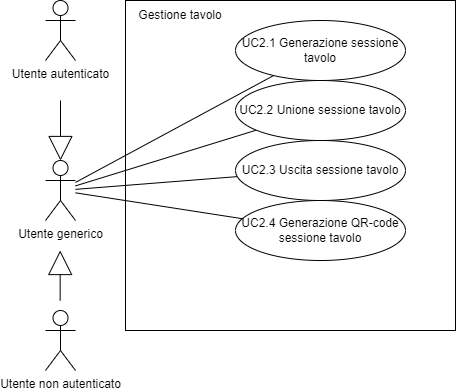
\includegraphics[scale=0.5]{usecase/tesi-uc21.drawio.png}
    \caption{Use Case - UC 2.1, UC 2.2, UC 2.3, UC 2.4}
\end{figure}
\begin{itemize}
    \item \textbf{Descrizione:} L'utente genera la sessione del tavolo.
    \item \textbf{Attore Primario:} Untente generico.
    \item \textbf{Precondizione:} L'utente si trova dentro la sezione gestione tavolo.
    \item \textbf{Postcondizione:} L'utente entra nella sessione generata del tavolo.
    \item \textbf{Scenrio principale:}
    \begin{itemize}
        \item L'utente si trova dentro la sezione gestione tavolo;
        \item L'utente clicca sul bottone crea sessione;
        \item Viene creata la sessione;
        \item L'utente viene inserito nella sessione creata.
    \end{itemize}
\end{itemize}
\subsection{UC2.2 - Unione sessione tavolo}
\begin{itemize}
    \item \textbf{Descrizione:} L'utente si unisce alla sessione del tavolo.
    \item \textbf{Attore Primario:} Untente generico.
    \item \textbf{Precondizione:} L'utente si trova dentro la sezione gestione tavolo.
    \item \textbf{Postcondizione:} L'utente entra nella sessione che è stata inserita.
    \item \textbf{Scenrio principale:}
    \begin{itemize}
        \item L'utente si trova dentro la sezione gestione tavolo;
        \item L'utente clicca sul bottone unisciti a una sessione;
        \item L'utente inserisce il numero della sessione;
        \item L'utente clicca sul bottone unisciti;
        \item L'utente viene inserito nella sessione.
    \end{itemize}
    % \item \textbf{Scenrio alternativo:}
    % \begin{itemize}
    %     \item L'utente si trova dentro la sezione gestione tavolo;
    %     \item L'utente clicca sul bottone unisciti a una sessione;
    %     \item L'utente inserisce il numero della sessione inesistente;
    %     \item L'utente clicca sul bottone unisciti;
    %     \item L'utente non viene inserito nella sessione.
    % \end{itemize}
\end{itemize}
\subsection{UC2.3 - Uscita sessione tavolo}
\begin{itemize}
    \item \textbf{Descrizione:} L'utente esce dalla sessione del tavolo.
    \item \textbf{Attore Primario:} Untente generico.
    \item \textbf{Precondizione:} L'utente si trova dentro la sezione gestione tavolo ed è dentro ad una sessione.
    \item \textbf{Postcondizione:} L'utente esce dalla sessione generata del tavolo.
    \item \textbf{Scenrio principale:}
    \begin{itemize}
        \item L'utente si trova dentro la sezione gestione tavolo;
        \item L'utente clicca sul bottone esci dalla sessione;
        \item L'utente viene rimosso dalla sessione.
    \end{itemize}
\end{itemize}
\subsection{UC2.4 - Generazione QR-code sessione tavolo}
\begin{itemize}
    \item \textbf{Descrizione:} L'utente genera il QR-code dalla sessione del tavolo per mostrarlo agli altri, che li permetterà di unire alla sessione direttamente scansionando il QR-code.
    \item \textbf{Attore Primario:} Untente generico.
    \item \textbf{Precondizione:} L'utente si trova dentro la sezione gestione tavolo ed è dentro ad una sessione.
    \item \textbf{Postcondizione:} L'utente genera il QR-code dalla sessione del tavolo.
    \item \textbf{Scenrio principale:}
    \begin{itemize}
        \item L'utente si trova dentro la sezione gestione tavolo;
        \item L'utente genera il QR-code della sessione;
        \item Vine mostrato il QR-code;
    \end{itemize}
\end{itemize}



\subsection{UC3 - Lista ordini}
\begin{figure}[H]
    \centering
    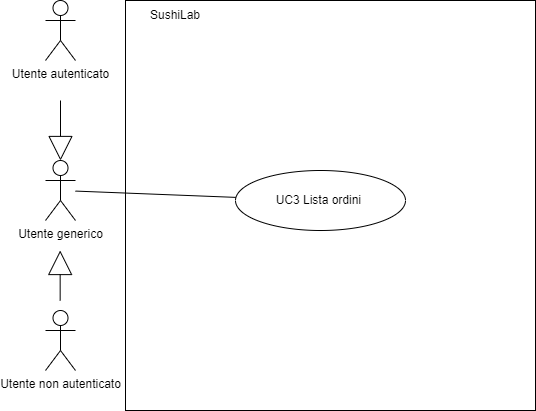
\includegraphics[scale=0.5]{usecase/tesi-uc3.drawio.png}
    \caption{Use Case - UC 3}
\end{figure}
\begin{itemize}
    \item \textbf{Descrizione:} L'utente visualizza la maschera di gestione ordini.
    \item \textbf{Attore Primario:} Untente generico.
    \item \textbf{Precondizione:} L'utente si trova dentro ad una sessione di tavolo.
    \item \textbf{Postcondizione:} Viene visualizzato la maschera di gestione ordini.
    \item \textbf{Scenrio principale:}
    \begin{itemize}
        \item L'utente si trova dentro il sistema con una sessione di tavolo attiva;
        \item L'utente clicca sul bottone lista ordini nella navbar;
        \item Viene mostrato la maschera di gestione ordini.
    \end{itemize}
\end{itemize}
\subsection{UC3.1 - Visualizza lista ordini del tavolo}
\begin{figure}[H]
    \centering
    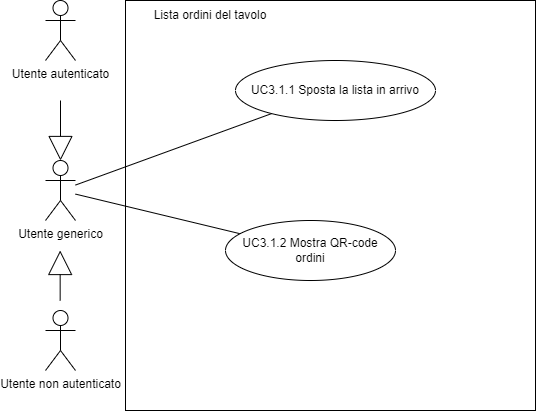
\includegraphics[scale=0.5]{usecase/tesi-uc311.drawio.png}
    \caption{Use Case - UC 3.1, UC 3.2, UC 3.3}
\end{figure}
\begin{itemize}
    \item \textbf{Descrizione:} L'utente visualizza la lista degli ordini della sessione di tavolo in cui si trova. 
    \item \textbf{Attore Primario:} Untente generico.
    \item \textbf{Precondizione:} L'utente si trova dentro la sezione lista ordini.
    \item \textbf{Postcondizione:} Viene visualizzato la lista degli ordini del tavolo.
    \item \textbf{Scenrio principale:}
    \begin{itemize}
        \item L'utente si trova dentro la sezione gestione ordini;
        \item L'utente clicca sul bottone "tavolo";
        \item Viene mostrato la lista dei piatti ordinati del tavolo.
    \end{itemize}
\end{itemize}
\subsection{UC3.2 - Visualizza lista ordini personali}
\begin{itemize}
    \item \textbf{Descrizione:} L'utente visualizzato la lista degli ordini personali.
    \item \textbf{Attore Primario:} Untente generico.
    \item \textbf{Precondizione:} L'utente si trova dentro la sezione lista ordini.
    \item \textbf{Postcondizione:} Viene visualizzato la lista degli ordini personali.
    \item \textbf{Scenrio principale:}
    \begin{itemize}
        \item L'utente si trova dentro la sezione gestione ordini;
        \item L'utente clicca sul bottone "personali";
        \item Viene mostrato la lista dei piatti ordinati dall'utente stesso.
    \end{itemize}
\end{itemize}
\subsection{UC3.3 - Visualizza lista ordini in arrivo}
\begin{itemize}
    \item \textbf{Descrizione:} L'utente visualizza la lista degli ordini in arrivo.
    \item \textbf{Attore Primario:} Untente generico.
    \item \textbf{Precondizione:} L'utente 
    \item \textbf{Postcondizione:} Viene visualizzato la lista lista degli ordini in arrivo.
    \item \textbf{Scenrio principale:}
    \begin{itemize}
        \item L'utente si trova dentro la sezione gestione ordini;
        \item L'utente clicca sul bottone "in arrivo";
        \item Viene mostrato la lista dei piatti in arrivo.
    \end{itemize}
\end{itemize}
\subsection{UC3.1.1 - Sposta la lista in arrivo}
\begin{figure}[H]
    \centering
    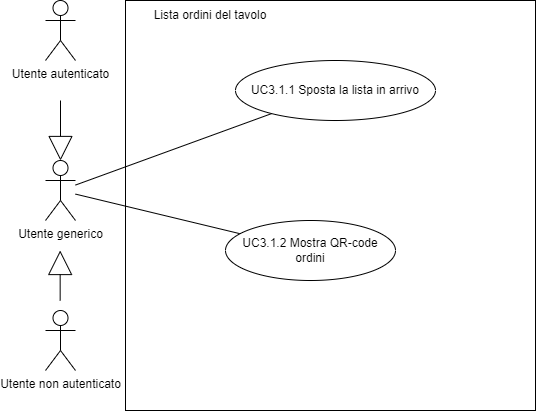
\includegraphics[scale=0.5]{usecase/tesi-uc311.drawio.png}
    \caption{Use Case - UC 3.1.1, UC 3.1.2}
\end{figure}
\begin{itemize}
    \item \textbf{Descrizione:} L'utente sposta la lista degli ordini in arrivo.
    \item \textbf{Attore Primario:} Untente generico.
    \item \textbf{Precondizione:} L'utente si trova dentro la sezione lista ordini del tavolo.
    \item \textbf{Postcondizione:} Viene spostato la lista degli ordini del tavolo in arrivo.
    \item \textbf{Scenrio principale:}
    \begin{itemize}
        \item L'utente si trova dentro la sezione gestione ordini del tavolo;
        \item L'utente clicca sul bottone sposta la lista in arrivo;
        \item Viene spostato la lista degli piatti ordinati personali in modalità dettaglio;
        \item Viene mostrato all'utente il messaggio "ordini spostati correttamente".
    \end{itemize}
\end{itemize}
\subsection{UC3.1.2 - Mostra QR-code ordini}
\begin{itemize}
    \item \textbf{Descrizione:} L'utente genera il QR-code della lista ordini per dopo mostrarlo al cameriere.
    \item \textbf{Attore Primario:} Untente generico.
    \item \textbf{Precondizione:} L'utente si trova dentro la sezione lista ordini del tavolo.
    \item \textbf{Postcondizione:} Viene mostrato il QR-code della lista degli ordini.
    \item \textbf{Scenrio principale:}
    \begin{itemize}
        \item L'utente si trova dentro la sezione gestione ordini del tavolo;
        \item L'utente clicca sul bottone QR-code;
        \item Viene generato il QR-code degli ordini;
        \item Viene mostrato il QR-code.
    \end{itemize}
\end{itemize}
\subsection{UC3.2.1 - Visualizza in dettaglio lista ordini personali}
\begin{figure}[H]
    \centering
    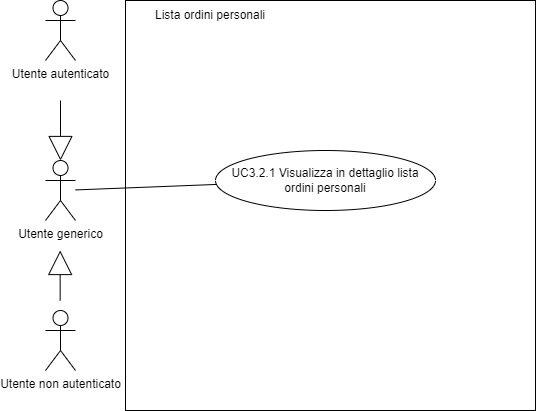
\includegraphics[scale=0.5]{usecase/tesi-uc322.drawio.png}
    \caption{Use Case - UC 3.2.1}
\end{figure}
\begin{itemize}
    \item \textbf{Descrizione:} L'utente visualizza la lista degli ordini personali in modalità dettaglio.
    \item \textbf{Attore Primario:} Untente generico.
    \item \textbf{Precondizione:} L'utente si trova dentro la sezione lista ordini personali.
    \item \textbf{Postcondizione:} Viene visualizzato la lista degli ordini personali con i piatti in modalità dettaglio.
    \item \textbf{Scenrio principale:}
    \begin{itemize}
        \item L'utente si trova dentro la sezione gestione ordini personali;
        \item L'utente clicca sul bottone "lente" con il +;
        \item Viene mostrato la lista dei piatti ordinati personali in modalità dettaglio.
    \end{itemize}
\end{itemize}
\subsection{UC3.3.1 - Ricezione piatto}
\begin{figure}[H]
    \centering
    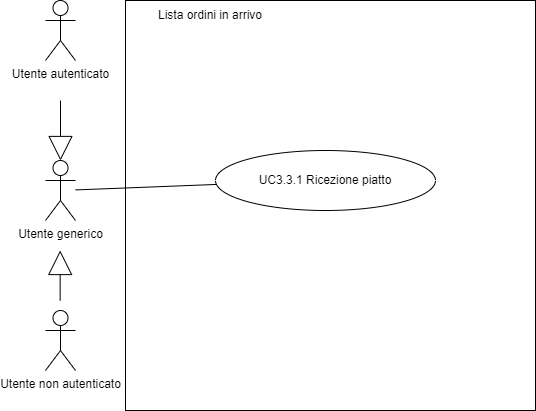
\includegraphics[scale=0.5]{usecase/tesi-uc333.drawio.png}
    \caption{Use Case - UC 3.3.1}
\end{figure}
\begin{itemize}
    \item \textbf{Descrizione:} L'utente marca un piatto in arrivo come ricevuto.
    \item \textbf{Attore Primario:} Untente generico.
    \item \textbf{Precondizione:} L'utente si trova dentro la sezione gestione ordini in arrivo e ha almeno un piatto nella lista in arrivo.
    \item \textbf{Postcondizione:} L'utente marca il piatto come arrivato diminuendo di 1 la sua quantità.
    \item \textbf{Scenrio principale:}
    \begin{itemize}
        \item L'utente si trova dentro la sezione gestione lista ordini in arrivo;
        \item L'utente clicca sul bottone "v" di un piatto;
        \item Viene diminuito di 1 la sua quantità.
    \end{itemize}
    \item \textbf{Scenrio alternativo:}
    \begin{itemize}
        \item L'utente si trova dentro la sezione gestione lista ordini in arrivo;
        \item L'utente clicca sul bottone "v" di un piatto con quantità uguale a 1;
        \item Viene diminuito di 1 la quantità del piatto e viene disabilitato il bottone.
    \end{itemize}
\end{itemize}

\section{Utente Non Autenticato}
\subsection{UC4 - Area personale}
\begin{figure}[H]
    \centering
    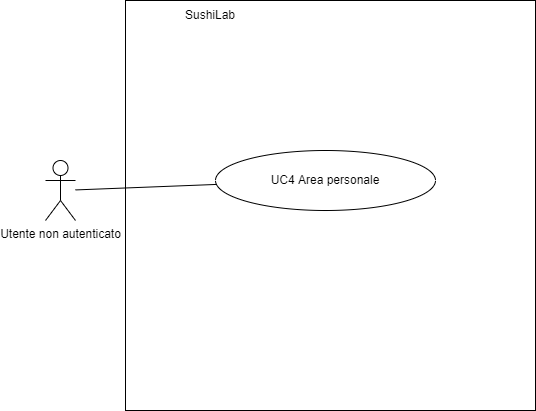
\includegraphics[scale=0.5]{usecase/tesi-uc4.drawio.png}
    \caption{Use Case - UC 4}
\end{figure}
\begin{itemize}
    \item \textbf{Descrizione:} L'utente visualizza la maschera dell'area personale.
    \item \textbf{Attore Primario:} Untente non autenticato.
    \item \textbf{Precondizione:} L'utente si trova dentro la web-app sushiLab.
    \item \textbf{Postcondizione:} Viene visualizzato la maschera dell'area personale.
    \item \textbf{Scenrio principale:}
    \begin{itemize}
        \item L'utente si trova dentro il sistema;
        \item Viene mostrato la mascheradell'area personale.
    \end{itemize}
\end{itemize}
\subsection{UC4.1 - Registrazione}
\begin{figure}[H]
    \centering
    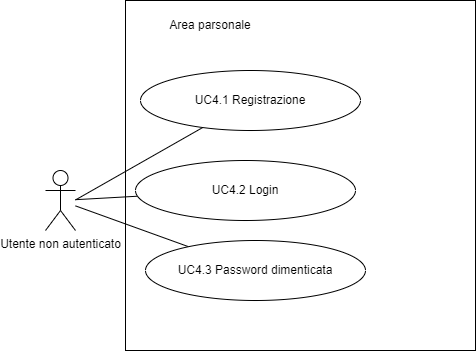
\includegraphics[scale=0.5]{usecase/tesi-uc41.drawio.png}
    \caption{Use Case - UC 4.1, UC 4.2, UC 4.3}
\end{figure}
\begin{itemize}
    \item \textbf{Descrizione:} L'utente viene registrato nella piattaforma.
    \item \textbf{Attore Primario:} Untente non autenticato.
    \item \textbf{Precondizione:} L'utente si trova dentro la web-app sushiLab.
    \item \textbf{Postcondizione:} Viene salvato i dati dell'utente inseriti durante la fase di registrazione nel data-base.
    \item \textbf{Scenrio principale:}
    \begin{itemize}
        \item L'utente si trova dentro l'area personale;
        \item L'utente clicca sul bottone registrati;
        \item Vine mostrato il form di registrazione;
        \item L'utente inserisce l'email;
        \item L'utente inserisce la password;
        \item L'utente ripete la password;
        \item L'utente clicca sul bottone registrati;
        \item Viene registrato correttamente l'account.
    \end{itemize}
    % \item \textbf{Estensioni:}
    % \begin{itemize}
    %     \item L'utente inserisce l'email già esistente nel data-base;
    %     \item Non viene registrato l'acocunt.
    % \end{itemize}
\end{itemize}
\subsection{UC4.2 - Login}
\begin{itemize}
    \item \textbf{Descrizione:} L'utente effettua login nella piattaforma.
    \item \textbf{Attore Primario:} Untente non autenticato.
    \item \textbf{Precondizione:} L'utente si trova dentro la web-app sushiLab.
    \item \textbf{Postcondizione:} Viene effettuato il login.
    \item \textbf{Scenrio principale:}
    \begin{itemize}
        \item L'utente si trova dentro l'area personale;
        \item L'utente inserisce l'email;
        \item L'utente inserisce la password;
        \item L'utente clicca sul bottone login;
        \item Viene effettuato il login correttamente.
    \end{itemize}
    % \item \textbf{Estensioni:}
    % \begin{itemize}
    %     \item L'utente inserisce l'email non esistente nel data-base o una password errata;
    %     \item Non viene effettuato il login.
    % \end{itemize}
\end{itemize}
\subsection{UC4.3 - Password dimenticata}
\begin{itemize}
    \item \textbf{Descrizione:} L'utente reimposta la password del proprio account.
    \item \textbf{Attore Primario:} Untente non autenticato.
    \item \textbf{Precondizione:} L'utente si trova dentro la web-app sushiLab.
    \item \textbf{Postcondizione:} Viene aggiornato la nuova password nel data-base.
    \item \textbf{Scenrio principale:}
    \begin{itemize}
        \item L'utente si trova dentro l'area personale;
        \item L'utente clicca sul bottone password dimenticata;
        \item Vine mostrato il form di recupero password;
        \item L'utente inserisce l'email;
        \item L'utente clicca sul bottone ottieni codice;
        \item L'utente arriva nel secondo form tramite il link mandato tramite email;
        \item L'utente inserisce la password;
        \item L'utente ripete la password;
        \item L'utente clicca sul bottone cambia password;
        \item Viene cambiato correttamente la password.
    \end{itemize}
    % \item \textbf{Estensioni:}
    % \begin{itemize}
    %     \item L'utente inserisce l'email non esistente nel data-base;
    %     \item Non viene effettuato il cambio password.
    % \end{itemize}
\end{itemize}
% \subsection{UCE1 - Email}
% \begin{itemize}
%     \item \textbf{Descrizione:} L'utente reimposta la password del proprio account.
%     \item \textbf{Attore Primario:} Untente non autenticato.
%     \item \textbf{Precondizione:} L'utente si trova dentro la web-app sushiLab.
%     \item \textbf{Postcondizione:} Viene aggiornato la nuova password nel data-base.
%     \item \textbf{Scenrio principale:}
%     \begin{itemize}
%         \item L'utente si trova dentro l'area personale;
%         \item L'utente clicca sul bottone password dimenticata;
%         \item Vine mostrato il form di recupero password;
%         \item L'utente inserisce l'email;
%         \item L'utente clicca sul bottone ottieni codice;
%         \item L'utente arriva nel secondo form tramite il link mandato tramite email;
%         \item L'utente inserisce la password;
%         \item L'utente ripete la password;
%         \item L'utente clicca sul bottone cambia password;
%         \item Viene cambiato correttamente la password.
%     \end{itemize}
% \end{itemize}
\section{Utente Autenticato}
\subsection{UC4.4 - Logout}
\begin{figure}[H]
    \centering
    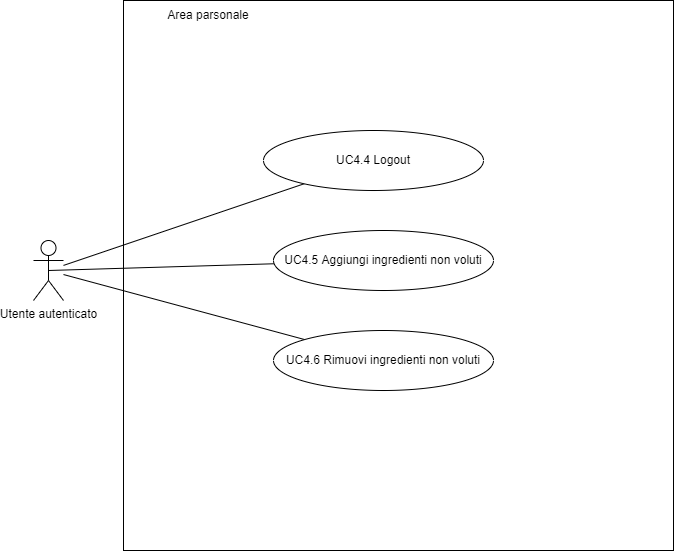
\includegraphics[scale=0.5]{usecase/tesi-uc42.drawio.png}
    \caption{Use Case - UC 4.4, UC4.5, UC4.6}
\end{figure}
\begin{itemize}
    \item \textbf{Descrizione:} L'utente effettua logout.
    \item \textbf{Attore Primario:} Untente autenticato.
    \item \textbf{Precondizione:} L'utente si trova dentro la web-app sushiLab ed ha effettuato la login.
    \item \textbf{Postcondizione:} Viene effettuato il logout.
    \item \textbf{Scenrio principale:}
    \begin{itemize}
        \item L'utente si trova dentro l'area personale;
        \item L'utente clicca sul bottone logout;
        \item Viene effettuato il logout dell'utente.
    \end{itemize}
\end{itemize}
\subsection{UC4.5 - Aggiungi ingredienti non voluti}
\begin{itemize}
    \item \textbf{Descrizione:} L'utente inserisce un ingrediente nella blacklist.
    \item \textbf{Attore Primario:} Untente autenticato.
    \item \textbf{Precondizione:} L'utente si trova dentro la web-app sushiLab  ha effettuato la login.
    \item \textbf{Postcondizione:} Viene inserito l'ingrediente nella blacklist.
    \item \textbf{Scenrio principale:}
    \begin{itemize}
        \item L'utente si trova dentro l'area personale;
        \item L'utente clicca sul bottone blacklist ingredienti;
        \item L'utente inserisce il nome del ingrediente;
        \item L'utente clicca sul bottone +;
        \item Viene inserito ingrediente nella blacklist.
    \end{itemize}
\end{itemize}
\subsection{UC4.6 - Rimuovi ingredienti non voluti}
\begin{itemize}
    \item \textbf{Descrizione:} L'utente rimuove un ingrediente dalla blacklist.
    \item \textbf{Attore Primario:} Untente autenticato.
    \item \textbf{Precondizione:} L'utente si trova dentro la web-app sushiLab  ha effettuato la login.
    \item \textbf{Postcondizione:} Viene rimosso l'ingrediente dalla blacklist.
    \item \textbf{Scenrio principale:}
    \begin{itemize}
        \item L'utente si trova dentro l'area personale;
        \item L'utente clicca sul bottone blacklist ingredienti;
        \item L'utente clicca sul bottone - di un ingrediente già esistente;
        \item Viene rimosso ingrediente dalla blacklist.
    \end{itemize}
\end{itemize}
\subsection{UC1.7 - Aggiungi preferiti}
\begin{figure}[H]
    \centering
    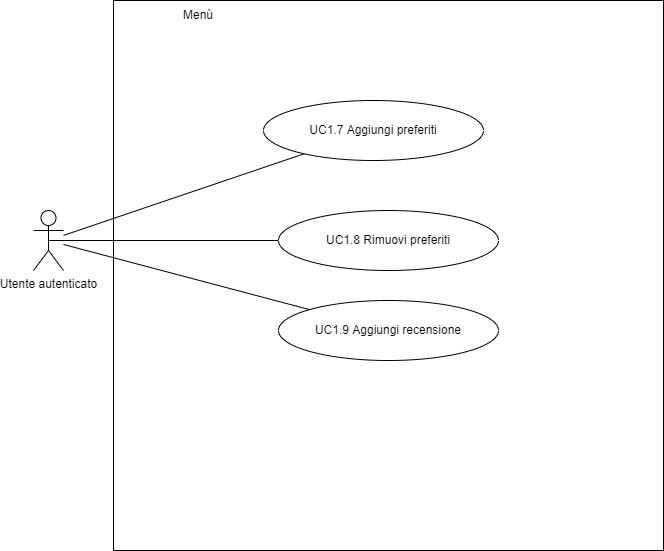
\includegraphics[scale=0.5]{usecase/tesi-uc111.drawio.png}
    \caption{Use Case - UC 1.7, UC1.8, UC1.9}
\end{figure}
\begin{itemize}
    \item \textbf{Descrizione:} L'utente aggiunge un piatto nella lista dei preferiti.
    \item \textbf{Attore Primario:} Untente autenticato.
    \item \textbf{Precondizione:} L'utente si trova dentro nella sezione menù, lista ordini personali o lista ordini in arrivo.
    \item \textbf{Postcondizione:} Viene inserito il piatto nei preferiti.
    \item \textbf{Scenrio principale:}
    \begin{itemize}
        \item L'utente si trova nella sezione menù, lista ordini personali o lista ordini in arrivo;
        \item L'utente clicca sul bottone "cuoricino grigio";
        \item Viene inserito il piatto nella lista dei preferiti.
    \end{itemize}
\end{itemize}
\subsection{UC1.8 - Rimuovi preferiti}
\begin{itemize}
    \item \textbf{Descrizione:} L'utente rimuove un piatto nella lista dei preferiti.
    \item \textbf{Attore Primario:} Untente autenticato.
    \item \textbf{Precondizione:} L'utente si trova dentro nella sezione menù, lista ordini personali, lista ordini in arrivo o lista preferiti.
    \item \textbf{Postcondizione:} Viene rimosso il piatto dalla lista dei preferiti.
    \item \textbf{Scenrio principale:}
    \begin{itemize}
        \item L'utente si trova nella sezione menù;
        \item L'utente clicca sul bottone "cuoricino rosa";
        \item Viene rimosso il piatto nella lista dei preferiti.
    \end{itemize}
\end{itemize}
\subsection{UC1.9 - Aggiungi recensione}
\begin{itemize}
    \item \textbf{Descrizione:} L'utente Aggiungi una recensione per un piatto.
    \item \textbf{Attore Primario:} Untente autenticato.
    \item \textbf{Precondizione:} L'utente ha selezionato un piatto e il piatto è in modalità dettaglio.
    \item \textbf{Postcondizione:} Viene aggiornato la recensione del piatto.
    \item \textbf{Scenrio principale:}
    \begin{itemize}
        \item L'utente ha selezionato un piatto e il piatto è in modificata dettaglio;
        \item L'utente clicca su una delle 5 stelle;
        \item Viene inserito la recensione del piatto.
    \end{itemize}
\end{itemize}
\subsection{UC5 - Visualizza lista preferiti}
\begin{figure}[H]
    \centering
    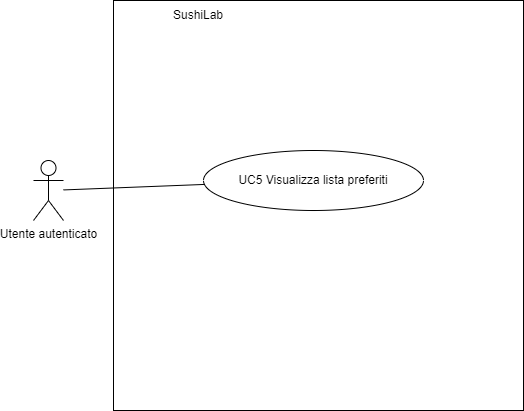
\includegraphics[scale=0.5]{usecase/tesi-uc5.drawio.png}
    \caption{Use Case - UC 5}
\end{figure}
\begin{itemize}
    \item \textbf{Descrizione:} L'utente visualizza la lista dei preferiti.
    \item \textbf{Attore Primario:} Untente autenticato.
    \item \textbf{Precondizione:} L'utente si trova dentro la web-app sushiLab ed ha effettuato la login.
    \item \textbf{Postcondizione:} Viene mostrato la lista dei preferiti.
    \item \textbf{Scenrio principale:}
    \begin{itemize}
        \item L'utente si trova dentro la web-app;
        \item L'utente entra nalla sezione lista preferiti;
        \item Viene mostrato la lista dei preferiti.
    \end{itemize}
\end{itemize}
% Durante la fase di analisi iniziale sono stati individuati alcuni possibili rischi a cui si potrà andare incontro.
% Si è quindi proceduto a elaborare delle possibili soluzioni per far fronte a tali rischi.\\

% \begin{risk}{Performance del simulatore hardware}
%     \riskdescription{le performance del simulatore hardware e la comunicazione con questo potrebbero risultare lenti o non abbastanza buoni da causare il fallimento dei test}
%     \risksolution{coinvolgimento del responsabile a capo del progetto relativo il simulatore hardware}
%     \label{risk:hardware-simulator} 
% \end{risk}

%**************************************************************
\section{Requisiti}
\subsection{Introduzione}
In base a quanto definito nell'analisi dei requisiti sono stati individuati una lista dei requisiti. Nella tabella si trovano tutti requisiti del progetto.
Il codice dei requisiti è così strutturato R(F/Q/V)(N/D/O) dove:
\begin{enumerate}
	\item[R =] requisito
    \item[F =] funzionale
    \item[Q =] qualitativo
    \item[V =] di vincolo
    \item[N =] obbligatorio (necessario)
    \item[D =] desiderabile
    \item[Z =] opzionale
\end{enumerate}
\subsection{Lista dei requisiti}
\begin{center}
    \rowcolors{2}{Cyan!10}{GreenYellow!10}
    \renewcommand{\arraystretch}{1.5}
    \begin{longtable}{ |p{1.5cm}|p{9cm}|p{1.5cm}|  }
        \hline
        \multicolumn{3}{|c|}{Tabella dei requisiti} \\
        \hline
        Codice&Requisito &Fonte \\
        \hline
        \endhead
        ROF1&L'utente può accedere al menù del ristorante&UC1 \\
        ROF2&All'utetne viene mostrato il menù del ristorante con tutte le categorie&UC1.1 \\
        ROF3&All'utetne viene mostrato il menù del ristorante con tutti piatti delle rispettive categorie di appartenenza&UC1.2 \\
        ROF4&L'utente può aumentare la quantità di un piatto nel menù&UC1.3 \\
        ROF5&L'utente può diminuire la quantità di un piatto nel menù&UC1.4 \\
        ROF6&L'utente può impostare la visualizzazione dei piatti del menù nella modalità dettaglio&UC1.5 \\
        ROF7&L'utente può impostare la visualizzazione dei piatti del menù nella modalità normale&UC1.6 \\
        ROF8&L'utente può accedere alla maschera per la gestione tavolo &UC2 \\
        ROF9&L'utente può generare la sessione del tavolo in cui si trova&UC2.1\\
        ROF10&L'utente può unirsi alla sessione di un tavolo&UC2.2 \\
        ROF11&L'utente può uscire dalla sessione di un tavolo&UC2.3\\
        ROF12&L'utente può generare il QR-code della sessione del tavolo in cui si trova&UC2.4\\
        ROF13&L'utente può accedere alla maschera per la gestione della lista ordini&UC3 \\
        ROF14&All'utetne viene mostrato la lista ordini del tavolo&UC3.1 \\
        ROF15&All'utetne viene mostrato la lista ordini personali &UC3.2 \\
        ROF16&All'utetne viene mostrato la lista ordini in arrivo&UC3.3 \\
        ROF17&L'utente può spostare la lista ordini del tavolo in arrivo &UC3.3.1 \\
        ROF18&L'utente può generare il QR-code della lista ordini del tavolo in cui si trova &UC3.1.2 \\
        ROF19&L'utente può impostare la visualizzazione dei piatti della lista ordini personali in modalità dettaglio&UC3.2.1 \\
        ROF20&L'utente può marcare un piatto della lista ordini in arrivo come ricevuto&UC3.3.1 \\
        ROF21&L'utente non autenticato può accedere all'area personale&UC4\\
        ROF22&L'utente non autenticato deve riuscire ad inserire email, password e conferma password nel form di registrazione per effettuare la registrazione &UC4.1\\
        ROF23&L'utente non autenticato deve riuscire ad inserire email e password nel form di login per effettuare la login &UC4.2\\
        ROF24&L'utente non autenticato deve riuscire ad inserire la email e la nuova password nel form del password dimenticata&UC4.3\\
        ROF25&L'utente autenticato deve riuscire ad effettuare la logout nell'area personale&UC4.4\\
        ROF26&L'utente autenticato può aggiungere ingredienti non voluti nell'area personale&UC4.4\\
        ROF27&L'utente autenticato può rimuovere ingredienti non voluti nell'area personale&UC4.4\\
        ROF28&L'utente autenticato può aggiungere un piatto nella lista dei preferiti&UC4.4\\
        ROF29&L'utente autenticato può rimuovere un piatto dalla lista dei preferiti&UC4.4\\
        ROF30&L'utente autenticato può aggiungere una recensione per un piatto&UC1.7\\
        ROF31&L'utente autenticato può visualizzare la propria lista dei preferiti&UC5\\
        ROV1&L'interfaccia utente del sistema dovrà essere sviluppato sfruttando il framework Angular&SyncLab\\
        ROV2&Lo stile dell'interfaccia utente del sistema dovrà essere sviluppato sfruttando CSS-3&SyncLab\\
        ROV3&Le chiamate API devono essere implementate tramite Stoplight&SyncLab\\
        ROV4&È necessario dividire le varie maschere in componenti diversi di Angular&SyncLab\\
        ROV5&La web-app dovrà funzionare sul browser Microsoft Edge dalla versione più recente&SyncLab\\
        ROV6&La web-app dovrà funzionare sul browser Google Chrome dalla versione più recente&SyncLab\\
        ROV7&La web-app dovrà funzionare sul browser Firefox dalla versione più recente&SyncLab\\
        ROV8&La web-app dovrà funzionare sul browser Safari dalla versione più recente&SyncLab\\
        RDV9&Il codice sorgente dovrà essere commentata&SyncLab\\
        ROQ1&Il codice sorgente della piattaforma sarà reperibile su GitHub&SyncLab\\
        ROQ2&Fornire una sezione tutorial che spieghi come si utilizza la web-app&SyncLab\\
\hline
\end{longtable}
\end{center}